\documentclass{article}

\PassOptionsToPackage{numbers,compress}{natbib}
\usepackage[dblblindworkshop]{neurips_2026}
\workshoptitle{Mechanistic Interpretability Workshop}

\usepackage[utf8]{inputenc}
\usepackage[T1]{fontenc}
\usepackage{amsmath}
\usepackage{amssymb}
\usepackage{amsthm}
\usepackage{booktabs}
\usepackage{graphicx}
\usepackage{microtype}
\usepackage{xcolor}
\usepackage{url}

\newtheorem{theorem}{Theorem}
\newtheorem{lemma}{Lemma}
\newtheorem{definition}{Definition}
\newtheorem{proposition}{Proposition}

\DeclareMathOperator{\softmax}{softmax}

\title{MINTS: Testing Strict Motif-Detector Claims in Nucleotide Transformers}

\author{Anonymous Authors}

\begin{document}

\maketitle

\begin{abstract}
Genomic foundation models often make biological labels linearly accessible, but decodability alone does not identify an internal mechanism. We study whether attention heads in nucleotide transformers can be justified as biological motif detectors under a strict mechanistic evidence standard. MINTS applies tokenization-aware QK/OV circuit analysis, residual-stream probing with controls, matched attention enrichment, activation patching, and sparse feature search to DNABERT-2 and a tested Nucleotide Transformer backend. Before making mechanistic claims, we report raw-sequence task baselines: GC-only AUROC ranges from 0.6361 to 0.9088, and 3--6-mer TF-IDF AUROC ranges from 0.7956 to 0.9406. DNABERT-2 layer-11 residual readouts achieve AUROC values of 0.9137, 0.9383, 0.8954, and 0.8847 on promoter and splice-site tasks, showing strong label decodability rather than a circuit-level explanation. Controls sharpen this interpretation: random-label and position-only probes are near chance; splice-site probes remain about 0.25 AUROC above GC-only controls; promoter probes are close to strong GC/k-mer baselines and should be interpreted cautiously. The primary strict test is negative: across 51,249 GM12878 CTCF sequences, no DNABERT-2 head meets the registered QK-to-motif criterion or matched attention-enrichment criterion. Batch activation patching finds promoter-TATA over-restoration and weaker splice-donor restoration, but these task-specific causal signals do not establish a CTCF motif-detector circuit. The results provide a calibrated evidence standard for nucleotide-transformer interpretability and show where representation-level success falls short of a strict motif-detector claim.
\end{abstract}

\section{Introduction}

Transformer models for nucleotide sequences now perform well on regulatory and splice-site prediction tasks \citep{ji2021dnabert,dallatorre2025nucleotide,jaganathan2019spliceai}. However, much of the usual evidence for biological understanding remains predictive or post hoc: attribution maps, motif visualizations, or probes can identify useful correlations, but they do not by themselves explain how internal computations produce predictions \citep{alipanahi2015deepbind,yu2024plantrna}. This distinction is central for mechanistic interpretability, where a claim about a component should survive direct tests of what it reads, where it attends, what it writes, and whether intervention on it changes the relevant behavior \citep{elhage2021framework,meng2022locating,heimersheim2024patching}.

Nucleotide transformers are a useful setting for this question. Known motifs give natural ground-truth hypotheses: a motif can specify where a component would need to attend, what feature it would need to read, and which perturbation should matter. They also expose a common interpretability risk. Attention maps, motif visualizations, and high probe scores can suggest a biological mechanism even when the model is using GC content, genomic-coordinate artifacts, distributed features, or another correlated signal. MINTS is designed to make the required evidence explicit.

The motifs used here are intentionally canonical. CTCF is a DNA-binding factor with a well-studied binding motif and public ENCODE peak calls in GM12878 cells, making it a natural strict test case for motif-local attention. The TATA box is a short promoter-associated sequence whose mutation gives a simple promoter perturbation. Splice donor and acceptor dinucleotides mark exon-intron boundaries and give compact sequence edits for task-level causal tests. These examples are not meant to exhaust regulatory biology; they are selected because a correct circuit-level claim should specify nucleotide support, token support, and an intervention target.

This paper contributes a calibrated evidence standard and a completed case study. MINTS separates three claims that are often conflated: residual decodability, task-level causal restoration under activation patching, and strict circuit-level motif detection. The primary strict test is CTCF: under the registered QK-alignment and matched-enrichment criteria, neither tested backend yields a CTCF attention head that should be called a strict motif detector. The promoter and splice analyses play a supporting role by showing that task labels can be decodable and that interventions can produce task-specific causal signals without establishing the stricter CTCF circuit claim.

\section{Related Work and Positioning}

Mechanistic interpretability of transformers has developed standard tools for decomposing attention heads, locating causal pathways, and tracing computational graphs \citep{elhage2021framework,meng2022locating,ameisen2025circuit}. QK/OV decomposition is especially relevant here because it separates where a head attends from what it writes. Activation patching then gives an intervention-based test of whether the component matters for a behavior \citep{heimersheim2024patching}. MINTS applies these established tools to genomic transformers with explicit motif-level criteria, using ground-truth motifs to test both positive circuit evidence and possible overinterpretation.

Genomic deep-learning interpretability has a different tradition. Models such as DeepBind, SpliceAI, DNABERT, GPN, and Nucleotide Transformer show that neural sequence models learn useful biological regularities \citep{alipanahi2015deepbind,jaganathan2019spliceai,ji2021dnabert,benegas2023gpn,dallatorre2025nucleotide}. Many analyses in this area focus on motif visualization, attribution, saliency, or downstream probing. These are valuable, but they usually do not establish an internal algorithm. A saliency map may highlight a motif, and a probe may decode a label, while the model's actual computation may depend on a distributed feature, a correlated composition signal, or a different component entirely.

MINTS is positioned between these literatures. It does not claim to solve genomic interpretability in general, and it does not treat a high downstream or probe score as mechanistic evidence. Instead, it asks a narrower question: when, if ever, is it justified to call a specific attention head a biological motif detector? This choice deliberately favors falsifiable criteria over narrative completeness. Negative results are therefore useful evidence, because they identify where an appealing mechanistic story is not supported by the implemented tests.

\section{Methods and Evidence Criteria}

\paragraph{Biology primer.}
Table~\ref{tab:biology-glossary} defines the biological and tokenization terms used in the evidence stack.

\begin{table}[t]
\caption{Glossary for mechanistic-interpretability readers.}
\label{tab:biology-glossary}
\centering
\scriptsize
\setlength{\tabcolsep}{3pt}
\resizebox{\textwidth}{!}{%
\begin{tabular}{@{}p{2.0cm}p{10.4cm}@{}}
\toprule
Term & Meaning in this paper \\
\midrule
Motif & A recurring DNA pattern associated with a biological function, such as transcription-factor binding or splice recognition. \\
PWM & Position weight matrix: a per-position nucleotide model used to score how well a DNA window matches a motif. \\
JASPAR & A public database of curated transcription-factor binding motifs; MINTS uses the MA0139.1 CTCF matrix. \\
CTCF & CCCTC-binding factor, a DNA-binding protein involved in chromatin organization and regulatory insulation. \\
TATA box & A short A/T-rich promoter element used here for promoter perturbation and patching tests. \\
Promoter & A regulatory DNA region near a gene start site that can influence transcription initiation. \\
Splice donor/acceptor & Boundary signals at the start and end of introns; donor sites usually contain GT and acceptor sites usually contain AG in genomic DNA. \\
Nucleotide token & A model input unit corresponding to one or more DNA characters after tokenization. \\
$k$-mer & A fixed-length DNA substring of length $k$, such as a 6-mer token. \\
BPE & Byte-pair encoding, a learned variable-length tokenizer; DNABERT-2 BPE tokens can cover different numbers of nucleotides. \\
\bottomrule
\end{tabular}
}
\end{table}

\paragraph{Transformer circuits.}
Let $\tau(x)=(t_1,\ldots,t_T)$ tokenize a nucleotide sequence into vocabulary items. The initial hidden state is
\begin{equation}
H^{(0)}_{j,:}=E_{\mathrm{tok}}[t_j,:]+P_{j,:}.
\end{equation}
For head $h$ in layer $l$, with hidden state $H^{(l-1)}$, the attention pattern is
\begin{equation}
A_h^{(l)}=\softmax\left(\frac{H^{(l-1)} W_h^Q (W_h^K)^T (H^{(l-1)})^T}{\sqrt{d_k}}\right),
\end{equation}
and the head output is $A_h^{(l)}H^{(l-1)}W_h^VW_h^O$. Following transformer-circuit notation \citep{elhage2021framework}, the QK circuit $W_h^Q(W_h^K)^T$ controls attention scores, while the OV circuit $W_h^VW_h^O$ controls what is written to the residual stream. For nucleotide models, tokenization matters: a motif position may correspond to one nucleotide token, a fixed $k$-mer token, or a learned BPE span.

\paragraph{Tokenization-aware motif support.}
The strict CTCF tests use nucleotide coordinates as ground truth and then map them to model-token coordinates. Let a motif hit span the half-open nucleotide interval $[a,b)$ and let token $j$ span $[u_j,v_j)$. Token $j$ supports the motif when
\begin{equation}
\max(0,\min(v_j,b)-\max(u_j,a))\geq 1,
\end{equation}
that is, when the token overlaps the motif interval by at least one nucleotide. Special tokens with zero-width offsets are retained for hidden-state alignment but receive no motif support. This rule is implemented in \texttt{src/motif\_scoring.py} and recorded in token-score manifests as \texttt{token\_support\_min\_overlap\_bp=1}.

\begin{center}
\fbox{\begin{minipage}{0.93\linewidth}
\small
\textbf{Sequence-to-token support mapping.}
\begin{enumerate}
\item Score each nucleotide window with the JASPAR CTCF PWM and mark motif windows above the deterministic support threshold.
\item Convert each motif window to a half-open nucleotide interval $[a,b)$.
\item Tokenize the same sequence with offsets, retaining zero-width special tokens for alignment.
\item Mark every token whose nucleotide interval overlaps $[a,b)$ by at least one base.
\item Use the resulting token-support intervals for QK/motif correlation and matched attention-enrichment tests.
\end{enumerate}
\end{minipage}}
\end{center}

\paragraph{Strict motif-detector criterion.}
An attention head is treated as a candidate biological motif detector only when three signals converge. It must assign elevated attention mass to motif-support positions, its QK scores must rank motif-support tokens above matched background tokens, and patching its activation must restore the task-relevant scalar in motif-destroying counterfactuals. The registered thresholds used here are in Table~\ref{tab:criteria}. These thresholds intentionally make attention alone insufficient.

\begin{table}[t]
\caption{Registered evidence criteria for candidate motif circuits. Thresholds are conservative screens: they are designed to prevent upgrading weak correlations, near-background attention, or unstable patching effects into motif-detector claims.}
\label{tab:criteria}
\centering
\small
\resizebox{\textwidth}{!}{%
\begin{tabular}{@{}llll@{}}
\toprule
Claim & Statistic & Threshold & Purpose and scale \\
\midrule
Motif localization & Attention enrichment ratio $\rho_h$ & $\rho_h \geq 2.0$ & Requires at least doubled motif-support attention over matched background. \\
Motif ranking & QK/motif Pearson correlation & $r \geq 0.5,\;p<0.05$ & Requires a large effect size, not merely significance from millions of tokens. \\
Causal importance & Patching metric $\mathrm{PM}(h,l)$ & $\mathrm{PM}\geq0.5$ & Requires at least half restoration of the clean-minus-corrupted target effect. \\
Strong causal importance & Same & $\mathrm{PM}\geq0.75$ & Marks stronger recovery while leaving room below exact full restoration. \\
Residual decodability & Probe AUROC or macro-$F_1$ & $\geq0.80$ or $+0.10$ & Establishes diagnostic readout quality, not circuit use by the model. \\
Robustness & Matched negative controls & No matched artifact & Requires simple controls not to explain the candidate signal. \\
\bottomrule
\end{tabular}
}
\end{table}

\paragraph{Activation patching.}
For a clean sequence $x_c$ and motif-destroyed corrupted sequence $x_{\mathrm{corr}}$, we patch a head output from the clean run into the corrupted run. The restoration metric is
\begin{equation}
\mathrm{PM}(h,l)=
\frac{f(x_{\mathrm{patched}})-f(x_{\mathrm{corr}})}
{f(x_c)-f(x_{\mathrm{corr}})},
\end{equation}
where $f$ is a scalar target such as a probe decision function or class logit. $\mathrm{PM}=0$ indicates no recovery, $\mathrm{PM}=1$ indicates full recovery of the clean effect, and values above one indicate over-restoration rather than simple full recovery \citep{heimersheim2024patching}.

\paragraph{Residual probes and controls.}
Linear probes are trained on frozen mean-pooled residual vectors. Their role is diagnostic: a high probe score establishes linear decodability, not that the probe direction is causal or used by the model. We therefore compare residual probes with GC-content-only classifiers, position-only classifiers where coordinates are available, GC-matched test subsets, shuffled-label probes, and GC-content distribution shifts. This framing follows linear-representation work while preserving the weaker interpretation that probes support \citep{park2024linear}.

\section{Experimental Setup}

The primary model is \texttt{zhihan1996/DNABERT-2-117M}, an encoder-style genomic transformer with learned BPE tokenization. The comparison backend is \texttt{InstaDeepAI/nucleotide-transformer-v2-100m-multi-species}, used as a tested fixed-6mer Nucleotide Transformer checkpoint \citep{dallatorre2025nucleotide}. The run exports DNABERT-2 QK and OV matrices for all 12 layers and 12 heads per layer, caches residual vectors for layers 0, 5, and 11, and uses custom Hugging Face forward hooks for attention-output patching because the installed TransformerLens path does not expose all required DNABERT-2 per-head tensors.

The residual-probe tasks are TATA promoter, non-TATA promoter, splice donor, and splice acceptor classification. The configured splits contain 5,062/212 train/test examples for TATA promoters, 30,000/1,372 for non-TATA promoters, and 30,000/3,000 for each splice task. The strict CTCF scan uses 51,249 prepared GM12878 CTCF peak sequences and the JASPAR MA0139.1 CTCF motif, aligned to exact overlapping DNABERT-2 BPE token spans. Batch patching uses motif-destroying clean/corrupted pairs for promoter-TATA and splice-donor tasks.

The current artifact does not include a fine-tuned DNABERT-2 sequence-classification head. To avoid treating probes as end-to-end model performance, we therefore report two raw-sequence predictive baselines before the mechanistic evidence: a GC-content logistic classifier using GC fraction, GC skew, and sequence length, and a TF-IDF 3--6-mer logistic classifier. Frozen DNABERT-2 residual readouts are shown beside these baselines only as representation context.

The pipeline writes small review-facing CSV, JSON, and figure artifacts while treating large activation, circuit-matrix, token-score, and sparse-autoencoder files as reproducible generated outputs. The full run takes about eight hours on the tested CUDA setup. The most expensive stages are the cross-model comparison and strict all-layer CTCF scans, so the appendix includes both full reproduction commands and a reduced smoke-run command for checking the code path on a smaller subset.

\section{Results}

\paragraph{Predictive performance context before mechanism.}
Table~\ref{tab:task-performance} separates task predictability from mechanistic evidence. The raw-sequence baselines are strong, especially on promoter tasks: a simple GC-content classifier already reaches 0.8955--0.9088 AUROC, and a 3--6-mer classifier reaches 0.9297--0.9406 AUROC. Splice tasks are less explained by composition alone, but k-mer baselines still recover substantial signal. The frozen DNABERT-2 layer-11 readout is included to show that the pretrained representation is predictive, but it remains a residual-decoding result, not a fine-tuned classifier-head result and not a circuit explanation.

\begin{table}[t]
\caption{Predictive task context before mechanistic analysis. GC-only and 3--6-mer rows are raw-sequence baselines. Frozen DNABERT-2 readout is a layer-11 residual classifier and is reported as diagnostic decodability evidence, not as end-to-end task performance.}
\label{tab:task-performance}
\centering
\scriptsize
\setlength{\tabcolsep}{3pt}
\resizebox{\textwidth}{!}{%
\begin{tabular}{@{}lrrrrrrrrr@{}}
\toprule
Task & Train & Test & GC AUROC & GC AUPRC & GC Acc. & k-mer AUROC & k-mer AUPRC & k-mer Acc. & DNABERT readout AUROC \\
\midrule
promoter\_tata & 5,062 & 212 & 0.8955 & 0.9040 & 0.8019 & 0.9297 & 0.9378 & 0.8255 & 0.9137 \\
promoter\_no\_tata & 30,000 & 1,372 & 0.9088 & 0.9218 & 0.8316 & 0.9406 & 0.9482 & 0.8652 & 0.9383 \\
splice\_sites\_donors & 30,000 & 3,000 & 0.6560 & 0.6892 & 0.6013 & 0.8185 & 0.8093 & 0.7430 & 0.8954 \\
splice\_sites\_acceptors & 30,000 & 3,000 & 0.6361 & 0.6343 & 0.5883 & 0.7956 & 0.7792 & 0.7220 & 0.8847 \\
\bottomrule
\end{tabular}
}
\end{table}

\paragraph{Residual decodability is strong but not uniformly clean.}
DNABERT-2 layer-11 residual probes exceed the registered residual-decodability threshold for all four tasks. Table~\ref{tab:probe-controls} combines headline AUROC values with the most important controls. Random-label probes collapse to chance, and position-only metadata does not explain the results. The splice-site tasks survive stronger checks: donor and acceptor residual probes remain about 0.25 AUROC above GC-only baselines on matched subsets and remain strong under GC shifts. The promoter tasks require caution because GC-only baselines are already high; their residual-probe advantage over GC-only controls is small on the matched comparison.

This distinction changes the interpretation of the headline probe table. The splice-site result is evidence that DNABERT-2's frozen residual stream contains linearly accessible information beyond simple GC composition or coordinate metadata. The promoter result is weaker mechanistically: it remains a valid decodability result, but the controls show that promoter-associated composition can explain much of the signal. This is why the paper avoids claiming that the promoter probes have isolated a clean causal promoter motif direction.

\begin{table}[t]
\caption{DNABERT-2 layer-11 probe-control summary. Numeric columns report AUROC; random-label values are means over eight shuffled-label runs.}
\label{tab:probe-controls}
\centering
\scriptsize
\setlength{\tabcolsep}{3pt}
\begin{tabular}{@{}lrrrrrr@{}}
\toprule
Task & Resid. & GC-only & Pos.-only & GC-match & Rand. & GC-shift range \\
\midrule
promoter\_tata & 0.9137 & 0.8956 & 0.4136 & 0.9137 & 0.4700 & 0.6182--0.8030 \\
promoter\_no\_tata & 0.9383 & 0.9088 & 0.3865 & 0.9383 & 0.5129 & 0.6312--0.8368 \\
splice\_sites\_donors & 0.8954 & 0.6560 & 0.4414 & 0.8944 & 0.5064 & 0.8432--0.8669 \\
splice\_sites\_acceptors & 0.8847 & 0.6361 & 0.4461 & 0.8838 & 0.5005 & 0.8573--0.8580 \\
\bottomrule
\end{tabular}
\end{table}

\begin{table}[t]
\caption{Target-alignment ledger. CTCF is the primary strict motif-detector chain. Promoter and splice results are auxiliary evidence for task-specific residual decodability and causal signal, not substitutes for a CTCF proof.}
\label{tab:target-alignment}
\centering
\scriptsize
\setlength{\tabcolsep}{2pt}
\resizebox{\textwidth}{!}{%
\begin{tabular}{@{}p{1.25cm}p{2.0cm}p{1.75cm}p{1.35cm}p{1.35cm}p{1.65cm}p{1.35cm}p{1.35cm}p{1.55cm}@{}}
\toprule
Target & Performance & Probe & QK & Enrichment & Patching & OV & SAE & Role \\
\midrule
CTCF & 51,249-sequence strict scan; no classifier target & No CTCF residual classifier used as strict evidence & Best $r=0.3004$; fail & Best $\rho_h=1.3130$; fail & No candidate promoted after failed QK/enrichment & No aligned OV claim & Best cosine 0.1158; weak & Primary strict chain \\
Promoter-TATA & GC 0.8955; k-mer 0.9297; readout 0.9137 AUROC & Decodable, but close to strong baselines & Not target-aligned in current artifact & Not target-aligned & Best $\mathrm{PM}=1.4029$; over-restores & L2H7 output cosine 0.1261; weak & Not promoter-specific & Auxiliary causal evidence \\
Splice donor & GC 0.6560; k-mer 0.8185; readout 0.8954 AUROC & Decodable beyond GC and k-mer & Not target-aligned in current artifact & Not target-aligned & Best $\mathrm{PM}=0.5485$; partial & Not audited & Not splice-specific & Auxiliary causal evidence \\
\bottomrule
\end{tabular}
}
\end{table}

\paragraph{The strict CTCF motif-detector test fails.}
The CTCF scan produced 281,915 motif-support tokens and 1,843,874 finite token positions after BPE span correction. Across all 144 DNABERT-2 heads, the best QK-to-motif correlation is $r=0.3004$, below the registered $r\geq0.5$ criterion. The best matched attention-enrichment ratio is $\rho_h=1.3130$, below the registered $\rho_h\geq2.0$ criterion. The tested Nucleotide Transformer backend also fails to recover a strict CTCF candidate, with best $r=0.0192$ and best $\rho_h=1.00009$. Thus, the tested fixed-6mer backend does not support the CTCF motif-local head hypothesis under the same criteria.

The negative CTCF result is not a failure of the pipeline; it is the point of using a registered evidence stack. With more than 1.8 million finite token positions, small correlations can be statistically nonzero while remaining too small to support a mechanistic claim. The all-layer enrichment scan similarly prevents a common attention-overinterpretation mistake: a head can have visible structure without assigning enough mass to matched motif-support positions to count as a motif-local detector.

\paragraph{Threshold sensitivity supports the conservative conclusion.}
Table~\ref{tab:threshold-sensitivity} and Figure~\ref{fig:threshold-sensitivity} summarize threshold sweeps over QK correlation, matched enrichment, and auxiliary patching metrics. Relaxing the QK threshold alone yields 31 heads at $r\geq0.1$, five at $r\geq0.2$, one at $r\geq0.3$, and none at $r\geq0.4$. Relaxing matched enrichment alone yields three heads at $\rho_h\geq1.1$, one at $\rho_h\geq1.25$, and none at $\rho_h\geq1.5$. The strict CTCF chain remains negative: no head jointly passes QK and enrichment once $r\geq0.2$, even with $\rho_h\geq1.1$, and the most permissive joint count at $r\geq0.1,\rho_h\geq1.1$ is two heads, equal to the 95th percentile of a permuted-head alignment null. The promoter and splice patching thresholds are more permissive because those are auxiliary task-specific interventions, not CTCF motif-detector proof.

\begin{table}[t]
\caption{Threshold sensitivity summary. Counts are heads passing each single-metric threshold, except the joint row, which requires both CTCF QK and enrichment. The permuted-head null shuffles enrichment-pass labels against QK-pass labels 1,000 times.}
\label{tab:threshold-sensitivity}
\centering
\scriptsize
\setlength{\tabcolsep}{3pt}
\resizebox{\textwidth}{!}{%
\begin{tabular}{@{}llrrrr@{}}
\toprule
Target & Sweep & Permissive count & Registered/strict count & Best value & Null reference \\
\midrule
CTCF & QK $r$ & 31 at $r\geq0.1$ & 0 at $r\geq0.5$ & 0.3004 & Motif-shuffle null requires per-token QK scores \\
CTCF & Enrichment $\rho_h$ & 3 at $\rho_h\geq1.1$ & 0 at $\rho_h\geq2.0$ & 1.3130 & Position-matched background mean $\rho_h\approx1.00$ \\
CTCF & Joint QK/enrichment & 2 at $r\geq0.1,\rho_h\geq1.1$ & 0 at $r\geq0.5,\rho_h\geq2.0$ & -- & Permuted-head 95th percentile is 2 at the permissive setting \\
Promoter-TATA & Patching $\mathrm{PM}$ & 40 at $\mathrm{PM}\geq0.25$ & 16 at $\mathrm{PM}\geq0.75$ & 1.4029 & Auxiliary task-specific signal \\
Splice donor & Patching $\mathrm{PM}$ & 3 at $\mathrm{PM}\geq0.25$ & 0 at $\mathrm{PM}\geq0.75$ & 0.5485 & Auxiliary task-specific signal \\
\bottomrule
\end{tabular}
}
\end{table}

\begin{table}[t]
\caption{Evidence ledger. Each row states the claim, the required evidence standard, the observed result, the supported interpretation, and the main limitation.}
\label{tab:evidence-ledger}
\centering
\scriptsize
\setlength{\tabcolsep}{2pt}
\resizebox{\textwidth}{!}{%
\begin{tabular}{@{}p{2.2cm}p{3.2cm}p{3.0cm}p{3.4cm}p{3.0cm}@{}}
\toprule
Claim & Required evidence & Observed result & Interpretation & Limitation \\
\midrule
Promoter and splice labels are decodable from DNABERT-2 residual states & Strong residual readout plus controls against trivial artifacts & Layer-11 AUROC range 0.8847--0.9383; random-label and position controls near chance & Residual states contain task-relevant information & Promoter tasks remain close to strong GC and k-mer baselines \\
Splice residual decodability is not explained by GC alone & Matched and shifted GC controls should preserve the readout advantage & Splice probes remain about 0.25 AUROC above GC-only matched controls & Stronger evidence for non-composition residual signal on splice tasks & Still a probe result, not a localized circuit \\
Promoter-TATA patching identifies task-specific causal signal & Head-level patching should restore a corrupted scalar target across many pairs & Best mean $\mathrm{PM}=1.4029$ over 327 usable pairs & A head can causally amplify the promoter-TATA readout under patching & Over-restoration and probe geometry prevent a simple full-recovery claim \\
Splice-donor patching identifies a weaker causal signal & Patching should restore a corrupted splice-donor scalar target & Best mean $\mathrm{PM}=0.5485$ over 500 usable pairs & Partial task-specific causal signal exists & Effect is small on average and not tied to QK/enrichment motif evidence \\
DNABERT-2 has a strict CTCF motif-detector head & One head should pass QK/motif ranking, motif-local enrichment, and causal evidence & Best QK $r=0.3004$; best $\rho_h=1.3130$; no passing candidate & The strict single-head CTCF detector claim is not supported & Negative result is scoped to selected model, motif scorer, data, and thresholds \\
Relaxed CTCF thresholds do not rescue the strict claim & Sensitivity sweep should reveal whether conclusions depend on the registered cutoffs & No joint QK/enrichment pass once $r\geq0.2$, even at $\rho_h\geq1.1$ & The negative CTCF conclusion is not an artifact of one conservative cutoff & Motif-shuffle and GC-matched nulls require raw artifacts not currently persisted \\
SAE and OV audits do not reveal a simple alternate CTCF circuit & Output-write or sparse features should align strongly with the biological target & TATA OV cosine 0.1261; CTCF SAE best cosine 0.1158 & Auxiliary audits remain consistent with a distributed or absent simple motif circuit & Audits are not exhaustive circuit discovery \\
\bottomrule
\end{tabular}
}
\end{table}

\begin{figure}[t]
\centering
\begin{minipage}{0.32\textwidth}
\centering
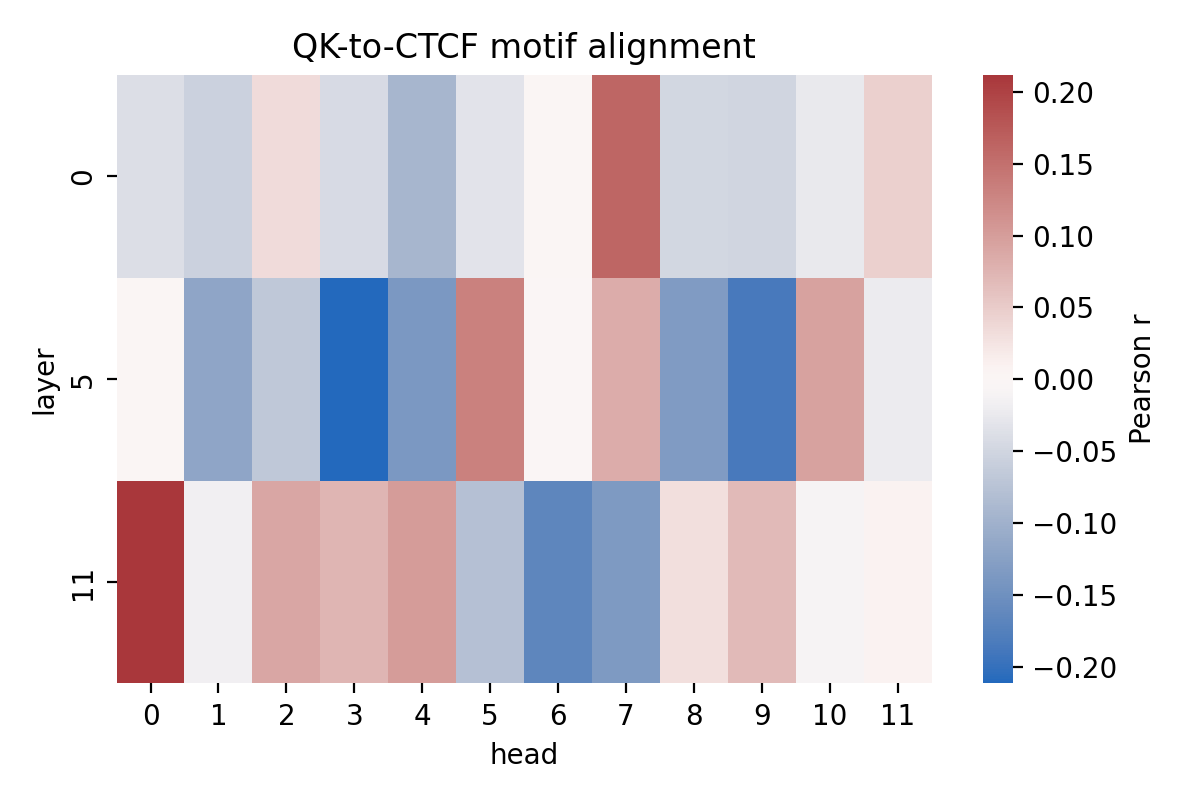
\includegraphics[width=\linewidth]{../results/figures/ctcf_qk_alignment_pearson_heatmap.png}
\end{minipage}
\hfill
\begin{minipage}{0.32\textwidth}
\centering
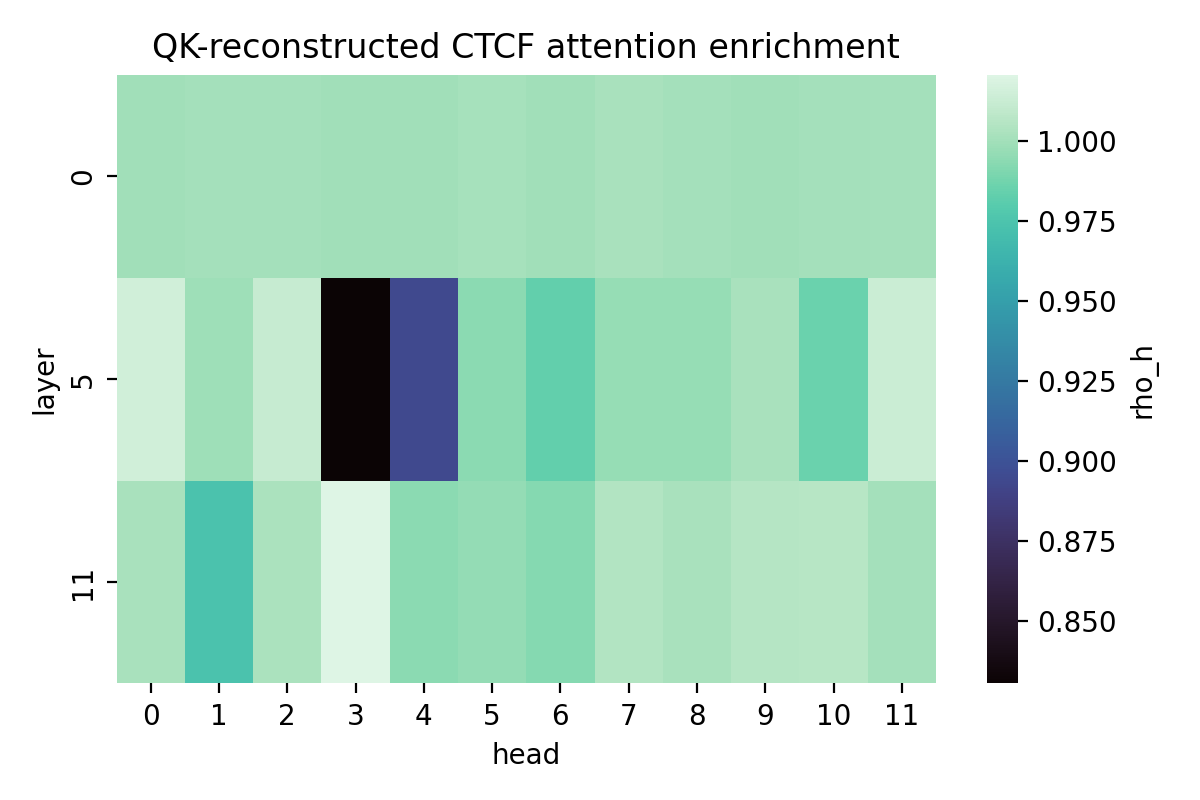
\includegraphics[width=\linewidth]{../results/figures/ctcf_qk_alignment_matched_attention_enrichment_rho_heatmap.png}
\end{minipage}
\hfill
\begin{minipage}{0.32\textwidth}
\centering
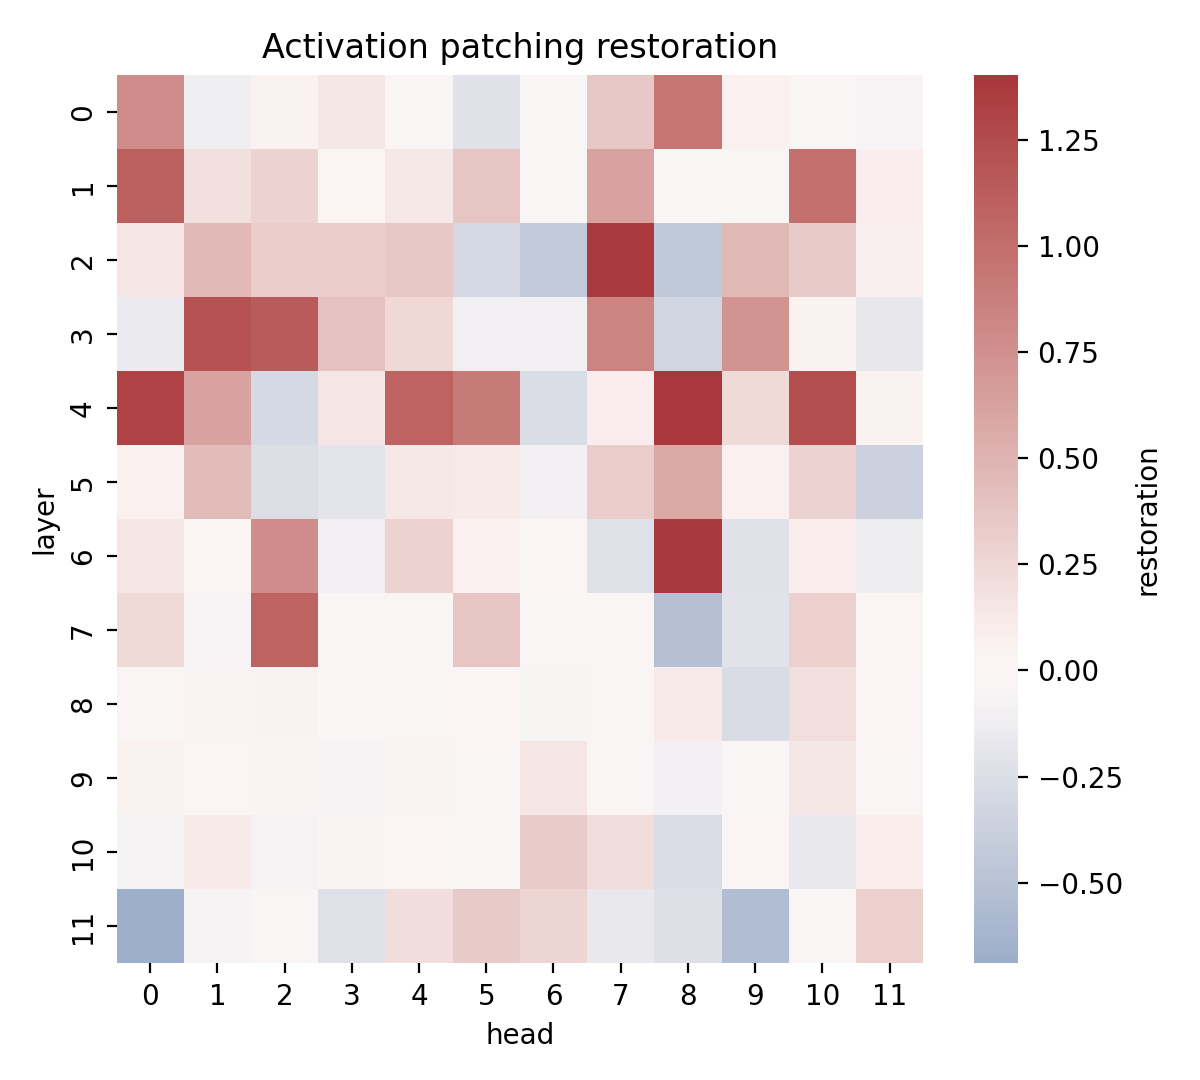
\includegraphics[width=\linewidth]{../results/figures/promoter_tata_batch_dnabert_activation_patching_heatmap.png}
\end{minipage}
\caption{Mechanistic evidence heatmaps. Left: DNABERT-2 CTCF QK-to-motif correlations. Middle: matched attention-enrichment ratios. Right: promoter-TATA batch patching. The CTCF heatmaps show a negative strict-proof result, while the TATA patching heatmap shows task-specific causal over-restoration.}
\label{fig:mechanistic-heatmaps}
\end{figure}

\begin{figure}[t]
\centering
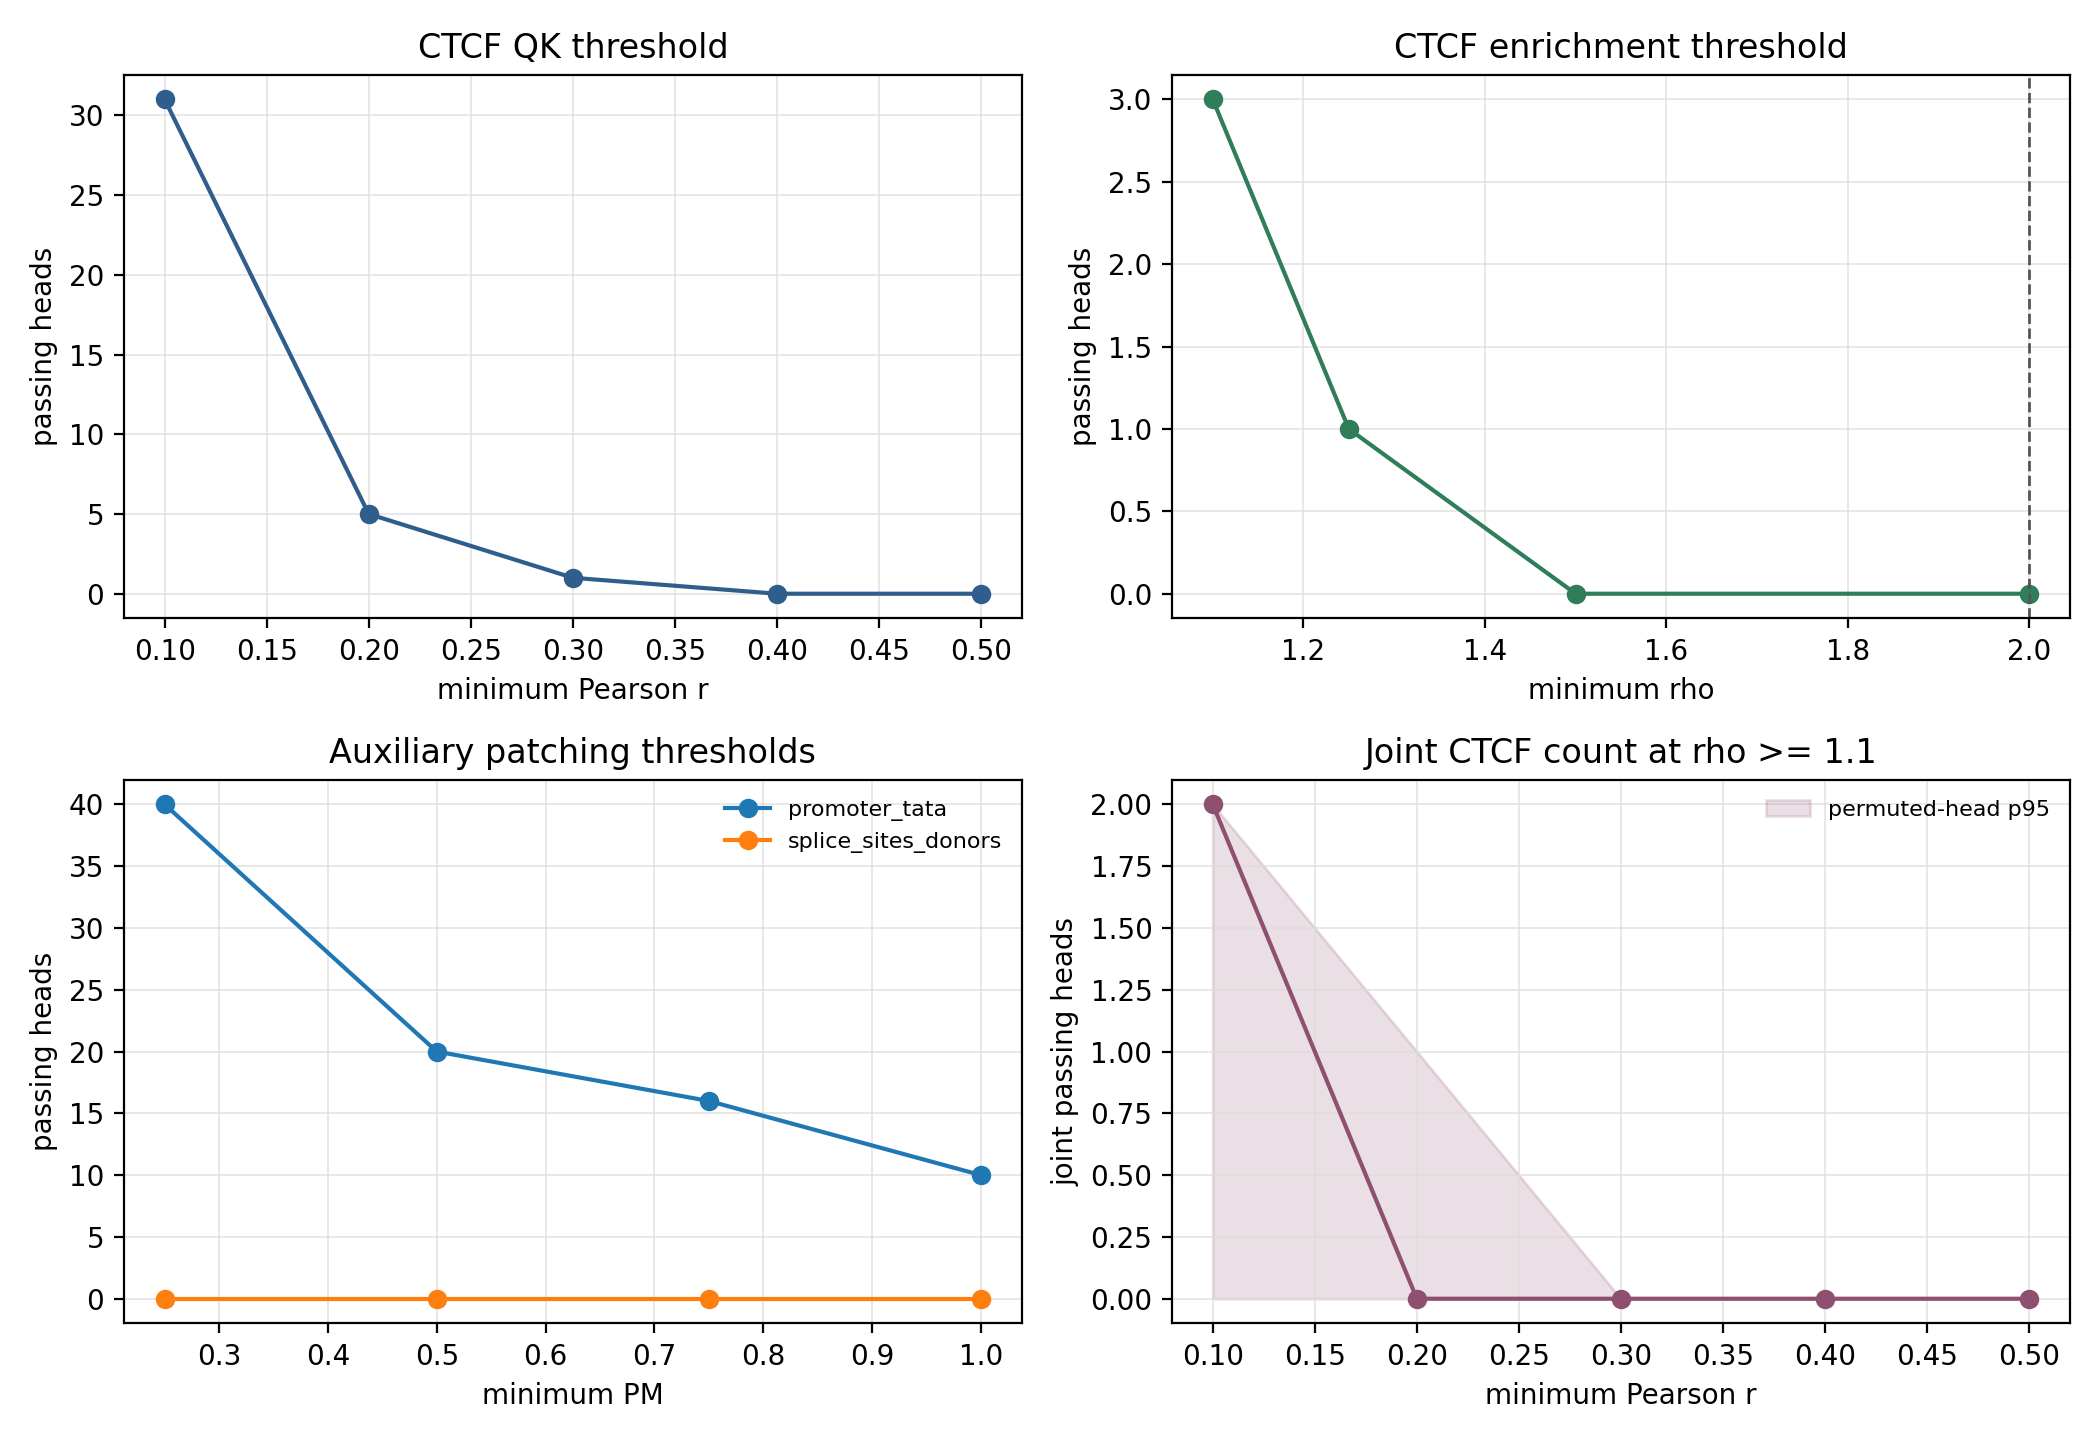
\includegraphics[width=\linewidth]{../results/figures/threshold_sensitivity.png}
\caption{Threshold sensitivity for QK alignment, matched attention enrichment, auxiliary patching, and joint CTCF QK/enrichment counts. Individual relaxed screens admit a small number of heads, but the strict CTCF chain remains negative under registered thresholds and under joint relaxation once $r\geq0.2$.}
\label{fig:threshold-sensitivity}
\end{figure}

\paragraph{Auxiliary promoter/splice patching gives task-specific causal signals.}
Batch promoter-TATA patching over 327 usable pairs identifies layer 4 head 8 with mean $\mathrm{PM}=1.4029$; layer 6 head 8 and layer 2 head 7 are also high. Because $\mathrm{PM}>1$ overshoots the clean-minus-corrupted effect, this is a methodologically sensitive causal signal rather than a simple full-recovery story. Batch splice-donor patching over 500 pairs identifies layer 1 head 8 with mean $\mathrm{PM}=0.5485$, a weaker but threshold-crossing effect. These interventions support task-relevant internal computation, but they do not identify a strict CTCF motif detector because the CTCF QK and enrichment screens have no passing head.

\paragraph{OV, SAE, and cross-model audits remain conservative.}
The TATA OV readout audit for layer 2 head 7 finds only weak alignment with the trained TATA probe direction: the top output-write singular-vector cosine is 0.1261 and the probe self-gain through the OV matrix is $-0.0326$. Sparse-autoencoder CTCF feature search is also weak, with best residual and MLP motif cosines of 0.0884 and 0.1158. In the protocol-level cross-model comparison, DNABERT-2 residual probes outperform the tested Nucleotide Transformer backend on the same tasks, but this is a checkpoint- and protocol-specific result, not a general claim about tokenization families or all Nucleotide Transformer variants.

\section{What This Teaches Mechanistic Interpretability}

The main lesson is that representation-level success and component-level mechanism are different claims. A residual probe can reveal that a biological label is linearly accessible while leaving open whether the model uses that direction, whether the feature is distributed, or whether the signal is driven by composition. Likewise, attention and motif visualizations can suggest a biological story without showing that a head's QK circuit ranks motif-support tokens or that intervention on the head changes the relevant behavior.

MINTS treats biological motifs as useful test cases precisely because they provide external ground truth. A motif defines nucleotide support, gives a concrete perturbation target, and lets us ask whether model-token support agrees with circuit behavior. The negative CTCF result is therefore informative rather than merely null: it shows that strict evidence stacks can prevent a plausible but unsupported motif-detector story. For mechanistic interpretability, the practical recommendation is to report claims at the level they are actually supported: decodability, task-specific causal signal, motif-local attention, or strict circuit-level motif detection.

\section{Limitations}

This study is intentionally scoped to small and medium genomic transformers and does not claim exhaustive explanation. Current large-model circuit-tracing work also emphasizes partial recovery of computation rather than complete mechanistic accounts \citep{ameisen2025circuit,lindsey2025biology}. The strict CTCF failure applies to the selected checkpoints, GM12878 CTCF intervals, JASPAR MA0139.1 motif scorer, BPE span-alignment rule, selected causal targets, and registered thresholds. It is not an impossibility theorem for all genomic transformers, all CTCF representations, all cell types, all motif scorers, or all circuit decompositions.

Linear probes remain limited evidence. They can reveal decodable information while exploiting correlated sequence composition, split artifacts, or metadata. The added GC, position, matched, random-label, and shift controls reduce this risk, especially for splice-site tasks, but promoter decodability remains entangled with GC composition. Activation patching is causal but incomplete: head-level restoration does not characterize the full circuit, and over-restoration can reflect denominator sensitivity, probe geometry, or out-of-distribution patched states. The threshold-sensitivity table reduces concern that the CTCF conclusion depends on one arbitrary cutoff, but it does not replace new data-generating null experiments. Finally, biological annotations are incomplete, and a single JASPAR PWM cannot represent all relevant regulatory mechanisms.

\section{Conclusion}

MINTS turns a common interpretability temptation into a falsifiable test: before calling an attention head a biological motif detector, require aligned QK scores, motif-local attention enrichment, and causal restoration. On DNABERT-2, promoter and splice-site labels are strongly linearly decodable from late residual states, and splice-site decodability survives simple composition and position controls. But the strict CTCF motif-detector proof fails across all tested heads, and the task-specific patching effects do not change that conclusion. The contribution is therefore both positive and negative: a reproducible evidence standard for nucleotide-transformer interpretability, and a concrete demonstration that strong representation-level decodability should not be upgraded into a circuit-level biological claim without stronger evidence.

\bibliographystyle{plainnat}
\bibliography{references}

\clearpage
\appendix

\section{Theoretical Details}

\begin{definition}[Biological Motif Detector]
An attention head $h$ in layer $l$ functions as a biological motif detector for motif $m$ if there exists a nonempty set of relevant query positions $\mathcal{Q}_m$ and a threshold $\tau$ such that, for each $i\in\mathcal{Q}_m$,
\begin{equation}
\mathbb{E}\left[\sum_{j\in\mathrm{supp}_m(x)} A_h^{(l)}[i,j]\mid \mathrm{supp}_m(x)\neq\varnothing\right]\geq\tau
\end{equation}
and the corresponding expectation conditioned on $\mathrm{supp}_m(x)=\varnothing$ is below $\tau$. Here $\mathrm{supp}_m(x)$ is the set of key positions whose local sequence windows instantiate motif $m$.
\end{definition}

\begin{theorem}[Layer-1 Motif Detection via QK Circuits]
Consider a layer-1 attention head operating on $H^{(0)}$. Let $s_m(j)$ denote a scalar motif score associated with key position $j$. If for a fixed query position $i$ there are constants $a_i\in\mathbb{R}$ and $\gamma>0$ such that
\begin{equation}
q_i^Tk_j=a_i+\gamma s_m(j)
\end{equation}
for all admissible key positions $j$, then the induced attention distribution is monotonically increasing in $s_m(j)$. If motif-bearing positions are separated from background positions by a positive margin in $s_m$, the head is a motif detector for $m$.
\end{theorem}

\begin{proof}
The attention logit is $\ell_{ij}=q_i^Tk_j/\sqrt{d_k}=a_i/\sqrt{d_k}+(\gamma/\sqrt{d_k})s_m(j)$. Since $\gamma/\sqrt{d_k}>0$, scaling preserves the ordering of motif scores. The exponential and softmax are strictly monotone in each logit when other logits are fixed, so positions with larger motif scores receive larger attention weights. A positive separation margin therefore induces an attention-mass threshold that separates motif-bearing from background positions.
\end{proof}

\begin{lemma}[Approximate Extension Under Linear Decodability]
Suppose that at layer $l-1$ there exists a vector $u_m$ such that
\begin{equation}
u_m^T h_j^{(l-1)}=s_m(j)+\epsilon_j,\qquad |\epsilon_j|\leq\delta.
\end{equation}
If a head's QK score is affine in this decodable direction and the clean motif/background score margin is greater than $2\delta$, then the attention ordering between motif and background positions is preserved.
\end{lemma}

\begin{proof}
For motif-bearing $j_m$ and background $j_b$, the score difference is proportional to $s_m(j_m)-s_m(j_b)+\epsilon_{j_m}-\epsilon_{j_b}$. The perturbation term lies in $[-2\delta,2\delta]$. A clean separation greater than $2\delta$ keeps the sign of the score difference fixed, so softmax preserves the motif/background ordering.
\end{proof}

\section{Implementation and Reproducibility Details}

The completed run started at 13:27:07 local time on April 14, 2026 and ended at 21:26:30 local time the same day. The manifest reports 28,760.213 seconds, or 7.989 hours. The longest steps were cross-model tokenization comparison, strict mechanistic proofs, and systematic causal intervention. The inspected result tree contains 125 files totaling about 4.71 GB, including CSV/JSON summaries, figures, NPZ archives, and sparse-autoencoder checkpoints.

The anonymized project repository is available at \url{https://anonymous.4open.science/r/MINTS/}. It contains the project code, configuration, local paper source, and reproduction instructions. The repository currently serves as the single source of truth for the submitted code; an explicit repository license has not yet been added.

The main reproduction commands are:
\begin{verbatim}
git clone https://anonymous.4open.science/r/MINTS/ MINTS
cd MINTS
python -m pip install -r requirements.txt
python main.py
python main.py --only-probe-controls
\end{verbatim}

A smaller smoke run is:
\begin{verbatim}
python main.py --max-probe-train 512 --max-probe-test 256
  --max-qk-alignment-sequences 128
  --max-cross-model-qk-alignment-sequences 128
  --max-feature-search-sequences 128 --sae-epochs 1
\end{verbatim}

Important verification artifacts include:
\begin{itemize}
\item \path{results/pipeline_run.json}
\item \path{results/tables/linear_probe_metrics.csv}
\item \path{results/tables/linear_probe_controls.csv}
\item \path{results/tables/downstream_task_performance.csv}
\item \path{results/tables/target_alignment_table.csv}
\item \path{results/tables/review_issue_matrix.csv}
\item \path{results/tables/evidence_ledger.csv}
\item \path{results/tables/threshold_sensitivity.csv}
\item \path{results/qk_alignment/ctcf_qk_alignment.csv}
\item \path{results/enrichment/ctcf_qk_alignment_matched_attention_enrichment.csv}
\item \path{results/patching/promoter_tata_batch_dnabert_activation_patching.csv}
\item \path{results/patching/splice_sites_donors_batch_dnabert_activation_patching.csv}
\end{itemize}
The heatmaps used in the paper are generated under \path{results/figures/}.

\section{Additional Results}

The full configured-split residual probe AUROCs are 0.9137 for TATA promoters, 0.9383 for non-TATA promoters, 0.8954 for splice donors, and 0.8847 for splice acceptors. The corresponding AUPRC values are 0.9241, 0.9475, 0.9049, and 0.8954.

\section{Response-to-Review Checklist}

Table~\ref{tab:review-triage} records the review issue matrix used to guide the revision. The anonymized reviewer IDs are treated as issue sources rather than as claims about reviewer intent.

\begin{table}[h]
\caption{Review issue matrix.}
\label{tab:review-triage}
\centering
\scriptsize
\setlength{\tabcolsep}{3pt}
\resizebox{\textwidth}{!}{%
\begin{tabular}{@{}p{1.0cm}p{2.2cm}p{4.0cm}p{4.6cm}p{1.8cm}@{}}
\toprule
ID & Issue & Concern & Resolution & Status \\
\midrule
mV6D & Clarity & Paper read as several analyses. & Abstract/introduction now state one calibrated evidence-standard claim; Results opens with task context and a target ledger. & Addressed \\
mV6D & Target mismatch & Promoter/splice evidence blurred into CTCF claims. & Promoter/splice patching is auxiliary; CTCF remains the strict chain. & Addressed \\
C5jL & Missing performance & Mechanistic claims lacked predictive context. & Added GC and 3--6-mer baselines plus frozen-readout context before mechanism. & Partial \\
C5jL & MI contribution & Venue contribution needed sharpening. & Contribution is now a falsifiable standard for motif-detector claims. & Addressed \\
C5jL & Thresholds & Registered thresholds need scale/sensitivity. & Added threshold purposes, sweeps, and available null calibration. & Addressed \\
ndFG & Undefined biology & Motifs and biological terms need more support. & Added motif rationale, glossary, and nucleotide-to-token support rule. & Addressed \\
ndFG & Limited scope & Conclusions could overstate selected models/motifs. & Limitations and target ledger state the scoped negative CTCF result. & Addressed \\
\bottomrule
\end{tabular}
}
\end{table}

\begin{table}[h]
\caption{Response-to-review checklist with exact fixes.}
\label{tab:response-checklist}
\centering
\scriptsize
\setlength{\tabcolsep}{3pt}
\resizebox{\textwidth}{!}{%
\begin{tabular}{@{}p{2.1cm}p{3.8cm}p{5.0cm}p{3.2cm}@{}}
\toprule
Concern & Exact fix & Where it appears & Artifact \\
\midrule
Writing clarity & Reframed the paper around one calibrated evidence-standard claim and one primary negative CTCF case study & Abstract, Introduction, target-alignment ledger, evidence ledger & \path{results/tables/evidence_ledger.csv} \\
Target mismatch & Separated CTCF strict motif-detector evidence from promoter/splice auxiliary decodability and patching evidence & Target-alignment table and evidence ledger & \path{results/tables/target_alignment_table.csv} \\
Missing performance context & Added GC and 3--6-mer raw-sequence baselines before mechanistic claims and kept frozen readouts labeled as residual decodability & Predictive performance context subsection & \path{results/tables/downstream_task_performance.csv} \\
Weak MI contribution & Stated the contribution as a falsifiable standard for motif-detector claims rather than broad genomic interpretability & Introduction, Related Work, and ``What This Teaches Mechanistic Interpretability'' & Manuscript text \\
Threshold justification & Added threshold purposes, sensitivity sweeps, and available null calibration & Criteria table and threshold-sensitivity subsection & \path{results/tables/threshold_sensitivity.csv} \\
Undefined biology & Added motif rationale, glossary, and nucleotide-to-token overlap rule & Introduction and Methods glossary/mapping block & \path{src/motif_scoring.py} \\
Limited scope & Strengthened limitations to selected checkpoints, intervals, scorer, tokenization rule, causal targets, and thresholds; removed impossibility framing & Limitations and Conclusion & Manuscript text \\
\bottomrule
\end{tabular}
}
\end{table}

For promoter-TATA batch patching, 327 token-shape-preserving pairs were usable with no near-zero denominator failures. The best mean score was layer 4 head 8 with $\mathrm{PM}=1.4029$, followed by layer 6 head 8 with $\mathrm{PM}=1.3791$ and layer 2 head 7 with $\mathrm{PM}=1.3642$. For splice donors, 500 pairs were usable with no denominator failures, and the strongest mean restoration was layer 1 head 8 with $\mathrm{PM}=0.5485$.

For the tested Nucleotide Transformer backend, residual-probe AUROCs were 0.6502, 0.6976, 0.5695, and 0.5647 on the same four tasks. DNABERT-2 therefore outperformed this backend by 0.2408--0.3259 AUROC in this protocol. This comparison should not be read as a general ranking of tokenizers or genomic transformer families.

\section{Declaration of LLM Usage}

LLM-assisted tools were used during the project for mathematical exposition refinement, debugging support, and code-generation drafts through Codex with state-of-the-art GPT-5.4/GPT-5.5-class models. The research direction, core problem decomposition, step-by-step implementation decisions, and final scientific interpretation were directed by the author. The author reviewed the generated code, checked it for errors and failure modes, corrected mistakes, and takes responsibility for the final manuscript, code, and claims.

\input{checklist}

\end{document}
